
\begin{figure*}[!ht]
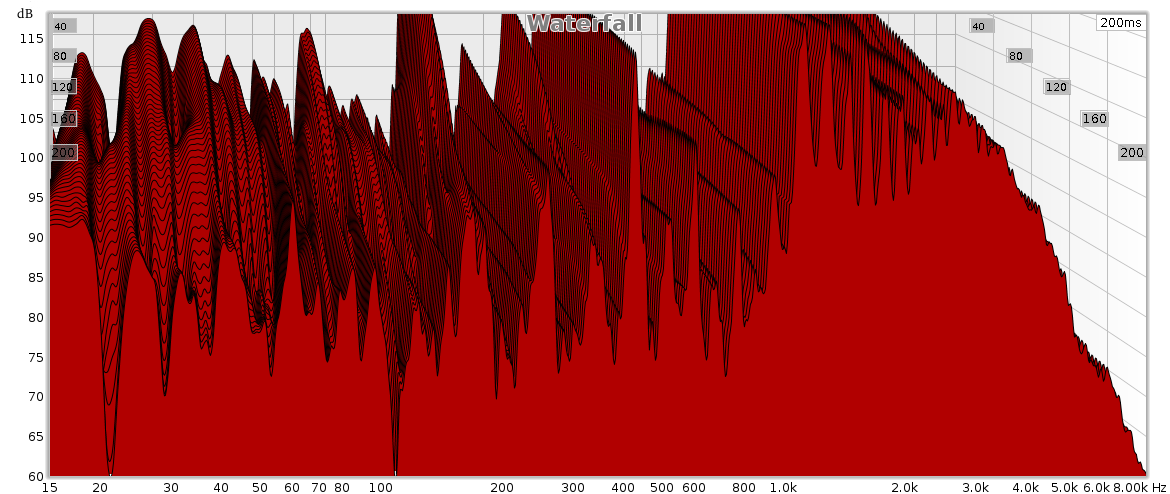
\includegraphics[width=\textwidth]{figs/waterfall} 
\caption{A waterfall plot of the \texttt{cartoon-spring.wav} from 0-200 ms between frequencies of 20-8000 Hz, where the height indicates the amplitude of each frequency. This plot was created with the REW tool~\cite{REWTool}.}
\label{fig:waterfall}
\end{figure*}

\section{Aural Distance}
\label{sec:distance}

As a distance metric, we used as a starting point the literature on acoustic fingerprinting~\cite{fingerprinting}.
Acoustic fingerprinting is the concept of creating a condensed, distinct summary of an audio file that can be used later to identify that audio file or to look it up in a database.
Acoustic fingerprints turn an audio file into a represent how the file will sound to the human ear regardless of how it is represented in a digital format~\cite{fingerprinting}.
There are numerous ways to develop acoustic fingerprints and companies like Shazam and Sound-Hound have developed complex algorithms to create accurate fingerprints even from low quality files recorded on a cellphone mic.
For this work, we used the work of Shazam~\cite{wang2003industrial} as an inspiration for our distance metric calculation.


As an intuition, the psycho-acoustic identity of a sound file (how humans distinguish between one sound and the next) can be captured by taking every ``moment'' of audio, and listing the predominate frequencies for that slice of time.
This intuition can be represented with a waterfall plot, as shown in Figure~\ref{fig:waterfall}, which plots how the frequencies change over time.
A waterfall plot uses the Fast Fourier Transform (FFT) to calculate many discrete Fourier transforms over small times slices.
In this way, a waterfall plot is a representation of an audio file as a list of spectrograms plotted over time.
In the Shazam method, the peaks are selected from each time slice of audio and used to create a ``constellation'' of peaks over time. 
This constellation is then used to build a hash that acts as a fingerprint to uniquely identify the audio sample.
We use a similar strategy by first performing a real Fast Fourier Transform on the audio file and then picking out the frequency peaks in each time frame.
However, the key difference in DSP-PBE is that we do not use the constellation as a hash for lookup in a database (as Shazam and SoundHound do), but instead, we need a distance metric between two constellations to provide a measure of how close we are to synthesizing the correct DSP filter.
Distance metrics are common in music synthesis tasks, for example, in the generation of jazz improvisations, where the improvisation should stay close by some measure to the original melody~\cite{donze2014machine}.

Fast Fourier Transforms (FFT) are the key to a good acoustic fingerprint.
The FFT, however, cannot be taken as a blackbox in our application.
The two factors we need to consider are 1) the window-size for how many samples will be used to calculate the FFT, and 2) the bin size which roughly speaking, defines the resolution of the FFT.

Each return element is a frequency \textit{bin}, and depending on the scale of your return array the size of these bins varies.
In order for each bin to correspond to 1 Hz the size of the return vector must be equal to the sampling frequency (44,100 Hz).
If each bin is not 1 Hz, the effects of spectral leakage will be seen.
This occurs when the bins do not correspond to the exact frequency peaks of the sound.
The amplitude from the peaks that fall in between bins will \textit{leak} over into the closest bin and create a distorted spectrogram.
For this reason we had to adjust the size of the FFT return arrays to be 44,100, as 44,100 Hz is a common format for audio.
Although this slows down the process of FFT, it provides the most accurate representation of the sound and for our purposes frequency accuracy is paramount.

With our constellations created from the waterfall plot, we constructed a \texttt{dist} function in measuring the aural distance and is faithful to the psycho-acoustics of the human ear.
Our implementation takes the Euclidean distance of the peaks in a time slice on the frequency-amplitude axis.
In order to define this distance more formally, we introduce the notation $c@t$ to indicate selecting time slice $t$ from constellation $c$.
We also use the function $peak:: Int \to Constellation \to Peak$ to select a peak from a constellation, where the peaks are in sorted order based on frequency.
Then, for an audio clip $x$ and an audio clip $y$, and a function $toC :: Audio \to Constellation$ to transform the audio clip into a constellation with $ts$ time slices and $p$ peaks in each time slice:

\begin{align*}
\sum_{t=0}^{ts}\ \sum_{i=0}^{p} euclid\Big(\ &peak(i,toC(x)@t), \\ &peak(i,toC(y)@t)\ \Big)
\end{align*}

Note that this definition requires the audio clips to be temporally aligned, which is not always a fair assumption in the real world. We leave the exploration of a temporal offset between two example audio samples to future work.

As a sanity check that this distance metric matches the psycho-acoustic definition of distance, we used the test cases listed in Table~\ref{table:dist}.

\begin{table*}[!h]
\centering
\begin{tabular}{|l | c | c|} 
 \hline
 Test Name \& Expected Result & Value 1 & Value 2 \\
 \hline
 \hline
 Identity & \multirow{2}{*}{(PianoC, PianoC) = 0} & \multirow{2}{*}{NA}\\ 
   \quad Value 1 = 0 &  & \\
 \hline
 Associativity & \multirow{2}{*}{(PianoC, PianoCSharp) = 5.635} & \multirow{2}{*}{(PianoCSharp, PianoC) = 5.635} \\
   \quad Value 1 = Value 2  & & \\
 \hline
 Associativity & \multirow{2}{*}{(PianoC, HornCSharp) = 20.500} & \multirow{2}{*}{(HornCSharp, PianoC) = 20.500} \\
   \quad  Value 1 = Value 2 & & \\
 \hline
 Filter less than pitch & \multirow{2}{*}{(PianoC, PianoFilterC) = 3.749} & \multirow{2}{*}{(PianoC, PianoCSharp) 5.635} \\ 
   \quad Value 1 $<$ Value 2 & & \\
 \hline
 Filter less than pitch+instrument & \multirow{2}{*}{(PianoC, PianoFilterC) = 3.749} & \multirow{2}{*}{(PianoC, HornCSharp) 20.500} \\
   \quad Value 1 $<$ Value 2 & & \\
 \hline
 Pitch less than pitch+instrument & \multirow{2}{*}{(PianoC, PianoCSharp) = 5.635} & \multirow{2}{*}{(PianoC, HornCSharp) 20.500} \\
   \quad Value 1 $>$ Value 2 & & \\
 \hline
\end{tabular}
\caption{Test cases to evaluate distance metric. The exact values are only important in relationship to the others.}
\label{table:dist}
\end{table*}


The goal in the synthesis procedure is to find a DSP filter program, $F$, such that \texttt{dist$(O, F(I))$ = 0}.
However, in practice the DSP-PBE Synthesizer can only get us so close to this metric and we instead just minimize this distance.
To do this, the user specifies a default threshold distance for the aural distance.
The threshold distance defines how close is acceptably close, and can be changed by the user depending on their needs or requirements.

